\documentclass[11pt]{article}
\usepackage[textwidth=18.0cm, textheight=23.0cm, top=2.0cm]{geometry}
\usepackage{pst-all}
\usepackage{amssymb}
\usepackage{tikz}
\usepackage{underscore}\begin{document}
\pagestyle{empty}


ClassName: \underline{\textbf{Class_03.2bp-1}}
\par
BinSize: \underline{\textbf{40 × 40}}
\par
ReduceSize: \underline{\textbf{40 × 40}}
\par
TypeNum: \underline{\textbf{19}}
\par
Num: \underline{\textbf{20}}
\par
OutS: \underline{\textbf{4800}}
\par
InS: \underline{\textbf{4169}}
\par
Rate: \underline{\textbf{0.869}}
\par
UB: \underline{\textbf{3}}
\par
LB0: \underline{\textbf{3}}
\par
LB: \underline{\textbf{3}}
\par
LBWithCut: \underline{\textbf{3}}
\par
NodeCut: \underline{\textbf{0}}
\par
ExtendedNodeCnt: \underline{\textbf{1}}
\par
GenNodeCnt: \underline{\textbf{1}}
\par
PrimalNode: \underline{\textbf{0}}
\par
ColumnCount: \underline{\textbf{3}}
\par
TotalCutCount: \underline{\textbf{0}}
\par
RootCutCount: \underline{\textbf{0}}
\par
LPSolverCnt: \underline{\textbf{1}}
\par
PricingSolverCnt: \underline{\textbf{0}}
\par
BranchAndBoundNum: \underline{\textbf{1}}
\par
isOpt: \underline{\textbf{true}}
\par
TimeOnPrimal: \underline{\textbf{0.000 s}}
\par
TimeOnPricing: \underline{\textbf{0.000 s}}
\par
TimeOnRmp: \underline{\textbf{0.062 s}}
\par
TotalTime: \underline{\textbf{0.125 s}}
\par
\newpage


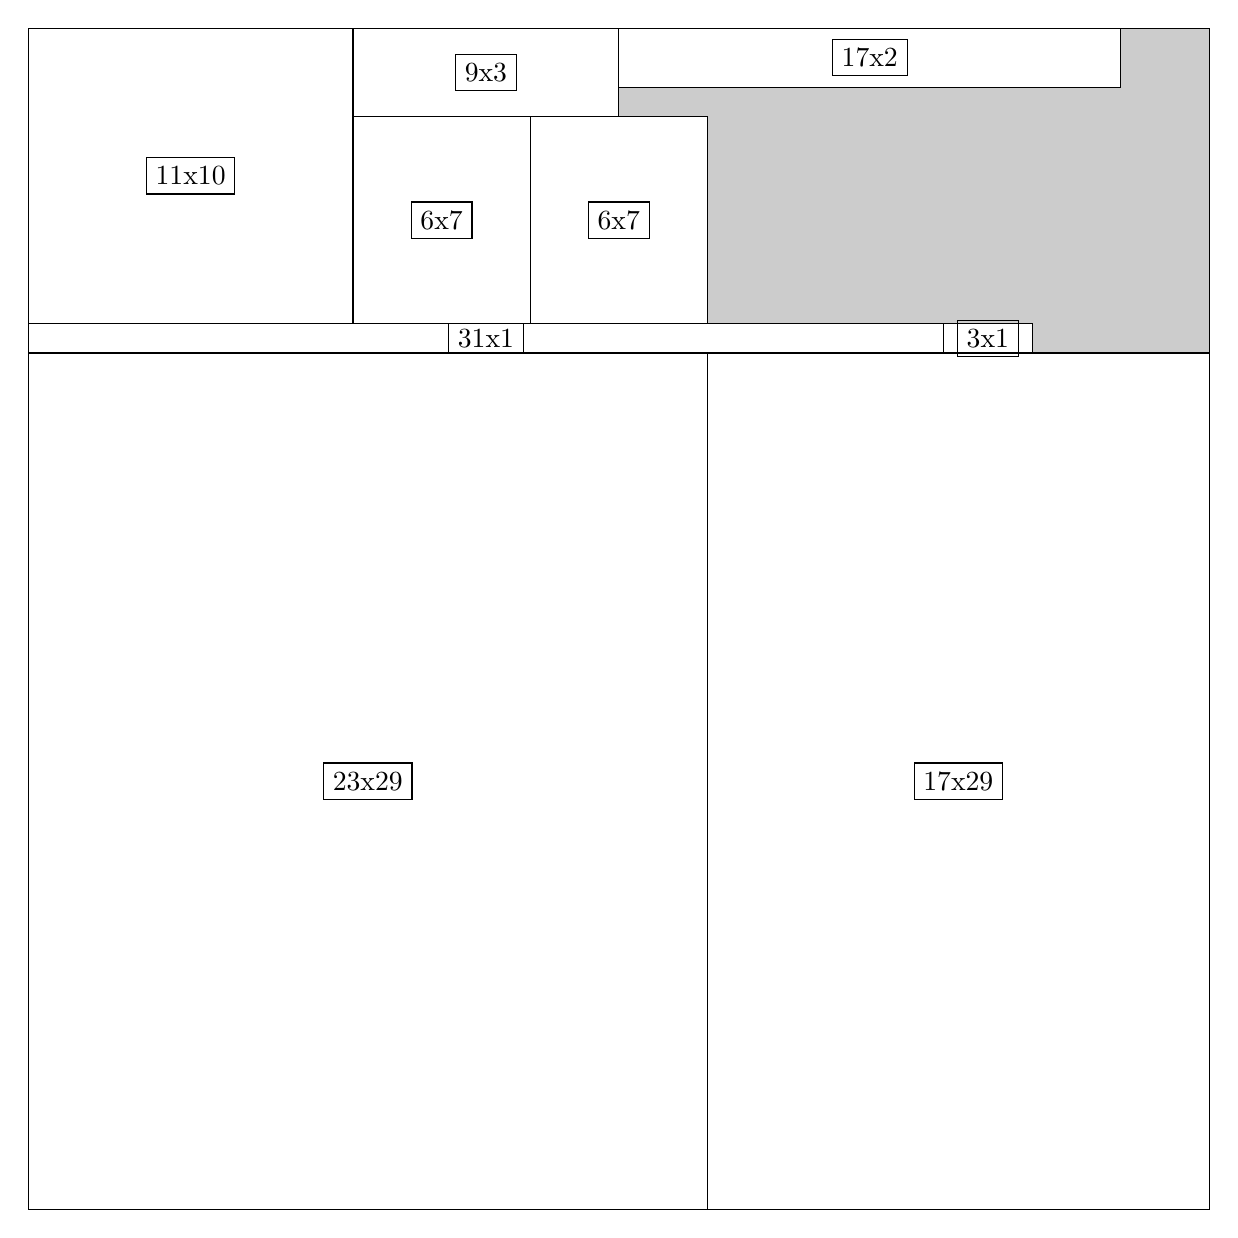
\begin{tikzpicture}[shorten >=1pt,scale=1.0,every node/.style={scale=1.0},->]
\tikzstyle{vertex}=[circle,fill=black!25,minimum size=14pt,inner sep=0pt]
\filldraw[fill=gray!40!white, draw=black] (0,0) rectangle (15.0,15.0);
\foreach \name/\x/\y/\w/\h in {31x1/0.0/10.875/11.625/0.375,6x7/4.125/11.25/2.25/2.625,11x10/0.0/11.25/4.125/3.75,6x7/6.375/11.25/2.25/2.625,23x29/0.0/0.0/8.625/10.875,17x29/8.625/0.0/6.375/10.875,17x2/7.5/14.25/6.375/0.75,9x3/4.125/13.875/3.375/1.125,3x1/11.625/10.875/1.125/0.375}
\filldraw[fill=white!40!white, draw=black] (\x,\y) rectangle node[draw] (\name) {\name} ++(\w,\h);
\end{tikzpicture}


w =31 , h =1 , x =0 , y =29 , v =31
\par
w =6 , h =7 , x =11 , y =30 , v =42
\par
w =11 , h =10 , x =0 , y =30 , v =110
\par
w =6 , h =7 , x =17 , y =30 , v =42
\par
w =23 , h =29 , x =0 , y =0 , v =667
\par
w =17 , h =29 , x =23 , y =0 , v =493
\par
w =17 , h =2 , x =20 , y =38 , v =34
\par
w =9 , h =3 , x =11 , y =37 , v =27
\par
w =3 , h =1 , x =31 , y =29 , v =3
\par
\newpage


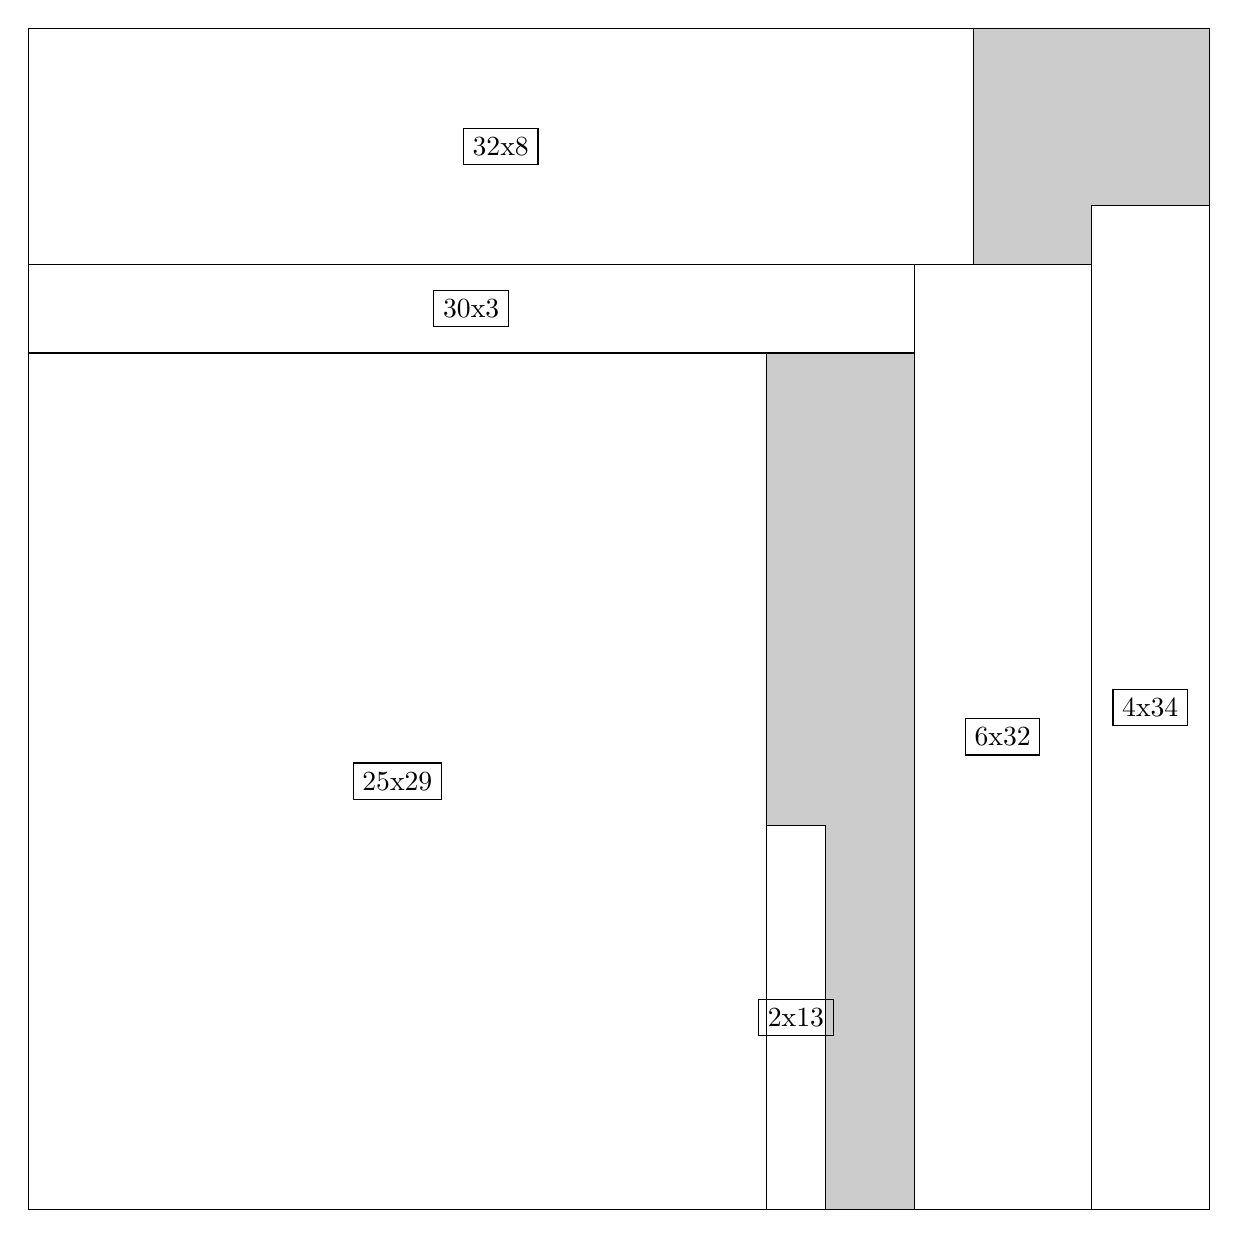
\begin{tikzpicture}[shorten >=1pt,scale=1.0,every node/.style={scale=1.0},->]
\tikzstyle{vertex}=[circle,fill=black!25,minimum size=14pt,inner sep=0pt]
\filldraw[fill=gray!40!white, draw=black] (0,0) rectangle (15.0,15.0);
\foreach \name/\x/\y/\w/\h in {30x3/0.0/10.875/11.25/1.125,32x8/0.0/12.0/12.0/3.0,6x32/11.25/0.0/2.25/12.0,4x34/13.5/0.0/1.5/12.75,25x29/0.0/0.0/9.375/10.875,2x13/9.375/0.0/0.75/4.875}
\filldraw[fill=white!40!white, draw=black] (\x,\y) rectangle node[draw] (\name) {\name} ++(\w,\h);
\end{tikzpicture}


w =30 , h =3 , x =0 , y =29 , v =90
\par
w =32 , h =8 , x =0 , y =32 , v =256
\par
w =6 , h =32 , x =30 , y =0 , v =192
\par
w =4 , h =34 , x =36 , y =0 , v =136
\par
w =25 , h =29 , x =0 , y =0 , v =725
\par
w =2 , h =13 , x =25 , y =0 , v =26
\par
\newpage


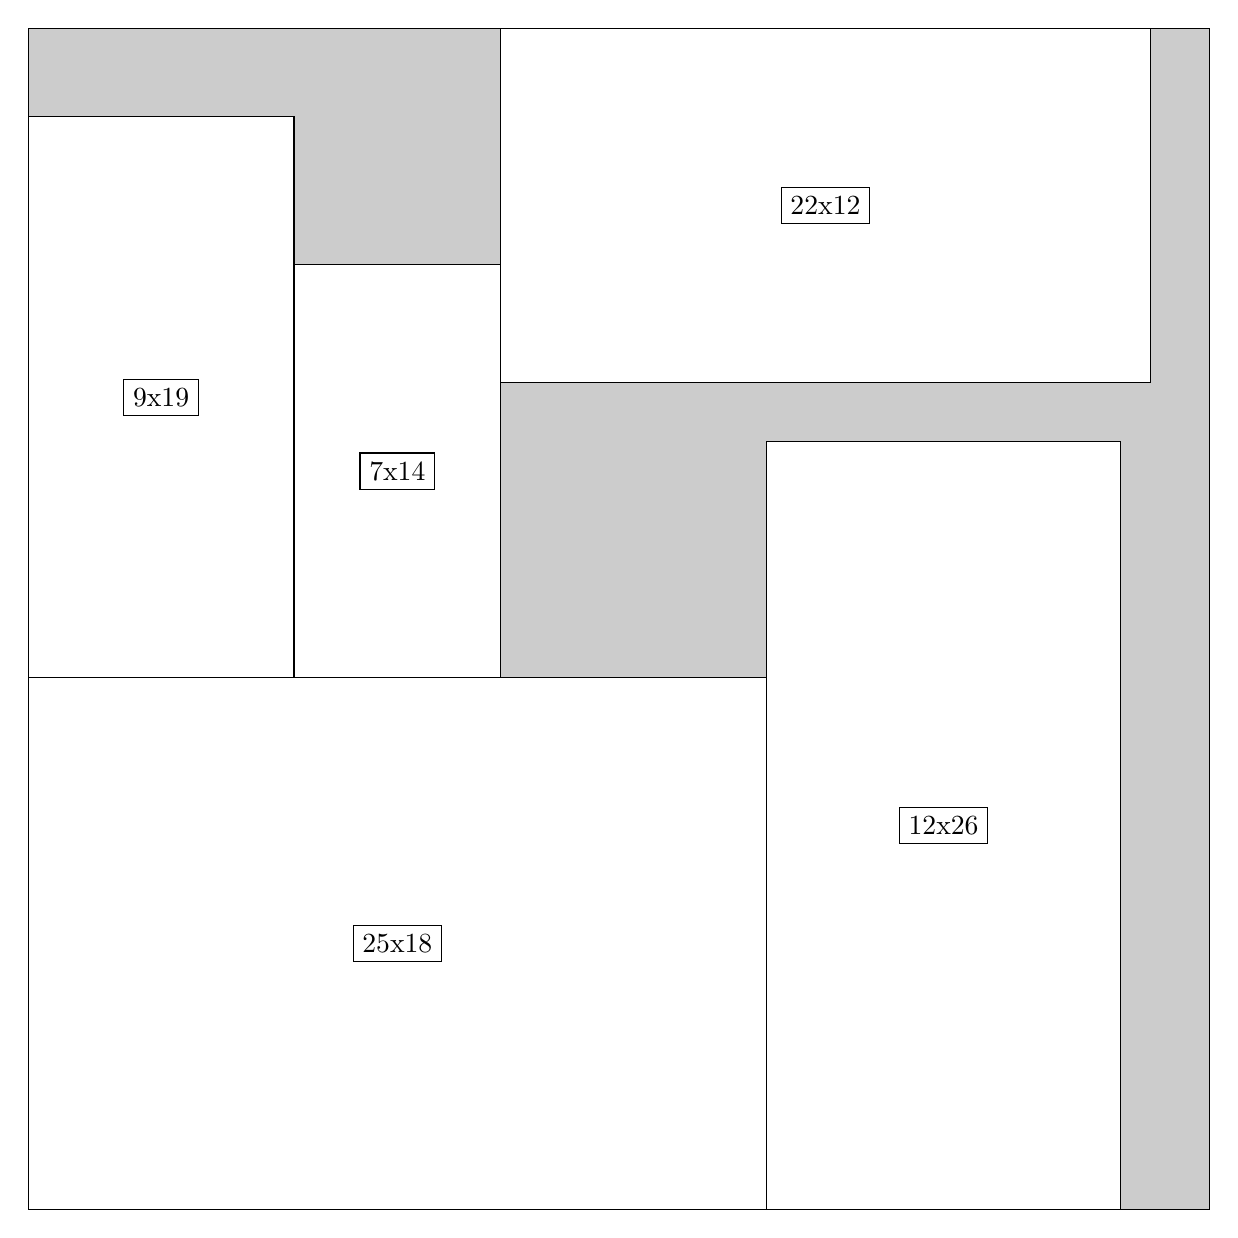
\begin{tikzpicture}[shorten >=1pt,scale=1.0,every node/.style={scale=1.0},->]
\tikzstyle{vertex}=[circle,fill=black!25,minimum size=14pt,inner sep=0pt]
\filldraw[fill=gray!40!white, draw=black] (0,0) rectangle (15.0,15.0);
\foreach \name/\x/\y/\w/\h in {25x18/0.0/0.0/9.375/6.75,12x26/9.375/0.0/4.5/9.75,22x12/6.0/10.5/8.25/4.5,9x19/0.0/6.75/3.375/7.125,7x14/3.375/6.75/2.625/5.25}
\filldraw[fill=white!40!white, draw=black] (\x,\y) rectangle node[draw] (\name) {\name} ++(\w,\h);
\end{tikzpicture}


w =25 , h =18 , x =0 , y =0 , v =450
\par
w =12 , h =26 , x =25 , y =0 , v =312
\par
w =22 , h =12 , x =16 , y =28 , v =264
\par
w =9 , h =19 , x =0 , y =18 , v =171
\par
w =7 , h =14 , x =9 , y =18 , v =98
\par
\newpage


\end{document}